\subsubsection{Buffer Design and Optimize}
Research shows that the organization of MapReduce
intermediate data is a challenge of design a  MapReduce library.
The organization of the Map output is critical to the
performance of many MapReduce applications, 
since the entier body of intermediate data must be
reorganized between the Map and Reduce phase:
Map produces data in the same order as the input,
while Reduce must consume data grouped by key.\cite{mao2010metis}
In a data center this operation is dominated by
the performance of the network, but when running 
on single multicore processor the performance
is dominated by the operations on the data structure
that holds intermediate data.
%已有的工作中,都有哪些buffer,都是如何实现的?

\begin{figure}[!h!t]  
    \centering
    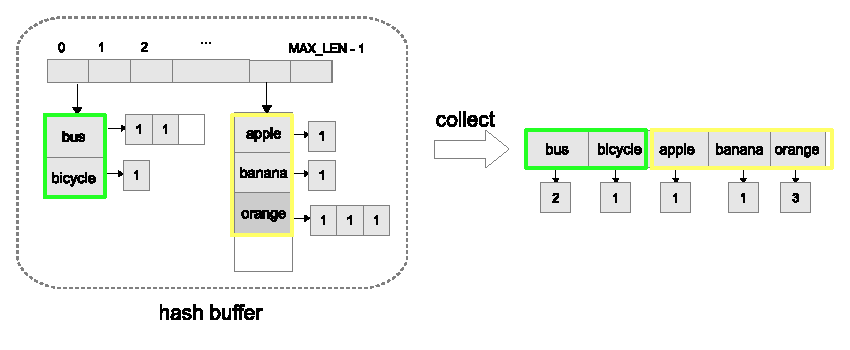
\includegraphics[width=0.5\textwidth]{eps/dmr_hash_buffer.eps}
    \caption{Produce-Consume model in SMR}
    \label{fig:dmr:hash-buffer}
\end{figure}
Defaultly, buffer in \myds is a hash table(Figure\ref{fig:dmr:hash-buffer}), 
and each element is a array of pointers to key arrays,
where the fixed is by a default value(256);
% When an intermediate key-value pair is generated
% by a map function,
% The hash function is applied to each key-value.
During the map phase, each map worker uses patition function
to index the buffer.
Once the buffer is determined, 
the element is indexed by the hash value of the key.
Inside each entry of a hash table,
\myds stores the key-value pairs in an array sorted by key.
If the hash table have enough entries, 
collisions will be rare and the key arrays will be short,
so that lookup and insert will have cost O(1).
The hash table's O(1) lookups 
make it particularly attractive for workloads with many repeated keys.
{\color{gray}(the reduce operator is immediately applied
to that pair based on the local container. This process is
performed using a combiner.)}

Hoverver, our producer-consumer model requires
reduce task is a contiguous block of memory, 
which implies that key-value of hash table should be gathered
before sending to reduce worker.
We address this issue by 
copying values out of the hash tables
at the end of the map phase and 
inserting them into a new contiguous array.
This extra copy is unfortunate and time-consuming.
Furthemore, it also requires frequent allocations and deallocations of memory 
along with the data structure creation and destrcution.

%为了提高效率,避免group阶段产生的开销,我们试图改进buffer的hash实现,它不再采用原来 Phoenix 中的 hash 表的组织方式,而是采用更简单的 array,map worker 产生的 key-value只需追加到 array 中即可,无需排序。

%The buffers are initially sized to a default value and then resized dynamically as needed.
To avoid the time-consuming collection in hash buffer, 
we implement a easy buffer, namely array buffer.
The buffers are initially sized to a default value and 
then reuse the buffer among sub-jobs.
It will indicate that the buffer is empty at the end of a sending, 
but will not free the memory until all map jobs have finished.
Each map thread could store its output 
by appending each key/value pair to array buffer, 
%Map阶段不需要进行排序,而是讲更多排序的工作move给reduce worker
and then as each sub-job is processed in turn,
the data structures and memory spaces 
for the input and intermediate data can be reused across the sub-job boundaries. 
This avoids the costs of expensive memory allocation and deallocation, 
as well as the data structures construction.
This could save the expensive operations 
such as concurrent memory allocations and deallocations,
as well as the building of data structures.
Furthemore, unlike hash buffer, array buffer is a contiguous block of memory,
it not need collection before send the buffer to channel.
For applications that likely have abundant duplicated keys (or values),
such as word\_count, it would be more worthwhile to use array buffer.

% For the array buffer implementation and no combiner in map phase,
% Map just need to . Thus, this technique is more effective
% for array buffer implementation than hash table buffer
% implementation.

%{\color{gray}(A related problem is that eager pipelining moves some of the
%sorting work from the mapper to the reducer.
%Recall that in the
%blocking architecture, map tasks generate sorted output: all the re-
%duce task must do is merge together the pre-sorted map output for
%each partition. In the eager pipelining design, map tasks send out-
%put records in the order in which they are generated, so the reducer
%must perform a full external sort. Because the number of map tasks
%typically far exceeds the number of reduces [4], moving more work
%to the reducer can degrade performance.
%)}




%applications of different buffer as table\ref{diff-buf}
%\begin{table}[]
%\centering
%\caption{My caption}
%\label{diff-buf}
%\begin{tabular}{|l|l|}
%\hline
%\multicolumn{2}{|l|}{\textbf{best buffer of applications}} \\ \hline
%\textbf{application}           & \textbf{buffer}           \\ \hline
%histogram                      & array                     \\ \hline
%word count                     & array                     \\ \hline
%linear regression              & hash                      \\ \hline
%string match                   & hash                      \\ \hline
%pca                            & hash                      \\ \hline
%\end{tabular}
%\end{table}
